\chapter{Software}
\label{methods}
\section{Computefarm}
\label{computefarm}
\subsection{Inspiration}
As discussed in Chapter \ref{background} global optimization solvers depend on the computational time, they also depend on fault tolerance of the objective function and resource consumption. In the event a black box function takes a long computational time, most global optimizations software offer parallel option. However, this is not beneficial when the function evaluation requires consumes a lot of resources to run the objective function. In this situation multiple function
evaluations are ran simultaneously thus increasing the amount of resources need by a multiple of number of objective functions running at the same time. When this occurs, the demand for resources from the optimization becomes higher than the machine can provide and causes what is known as \textit{resource contention}. 
  This is where the motivation of computefarm comes from, a software application to parallelize global optimization solvers by distributing function evaluations to client computers. By distributing the evaluations out to client computers the resource contention is minimal and a number of search space points are evaluated simultaneously. Another feature of computefarm is that it handles failures in the client machines. If a client disconnects or
  fails to run the function evaluation, computefarm handles the failure by reassigning the evaluation to another client in hopes of success. This is more beneficial than on a single machine facing a failure that causes the whole optimization process to stop and to restart again. In some optimization cases this can be months of computational time lost due to a single failure. By using Computefarm for global optimization algorithms, the user is able to run the program in parallel, avoid high
  resource contention and obtain fault-tolerance in the function evaluations.   
  
\subsection{Requirements}
Computefarm is a distributed system to send out tasks to multiple client computers. In the case of global optimization a server distributes function evaluations to client computers. To keep overhead of using Computefarm to a minimal only three requirements are needed to run Computefarm, they are
\begin{itemize}
    \item port number for socket connection (User provided),
    \item the runnable objective function script name (User provided), and
    \item list of population points to evaluate the objective function at on client machines (global optimization algorithm provided).
\end{itemize}
The first two points are passed into the solver and further passed to Computefarm for the initialization phase. The last point is passed in by the algorithm due to the metric it uses to determine which points in the domain of the objective function should be evaluated at each iteration step.  
\subsection{Structure}
 The implementation of computefarm is based on the client-server model, such that the software farms unused or accessible client machines to wait upon tasks directed by the server machine. For global optimization this means the server delegates points in the search space to the client computers to evaluate a black box function. The clients then return the result to the server machine and wait on further positions to evaluate. The server then a provides a list of
  results to the
  global optimization solver from each evaluated point. 
  In the case of a failure the server will receive a disconnect from the client machine then places the position back into the queue of positions needing to be evaluated. The server will later then provide the position to a client that is waiting on a new point to evaluate. This ensures fault tolerance in the computefarm software such that the global optimization solver does not need to restart if a client computer fails.  
  An extra step is taken in Computefarm where client machines are reawakened to ensure the maximum number of client machines are available to be utilized by the server. 
  Figure \ref{fig:computefarm} shows the flow of a global optimization algorithm using Computefarm. 
\clearpage
\begin{figure}[h!]
    \centering
    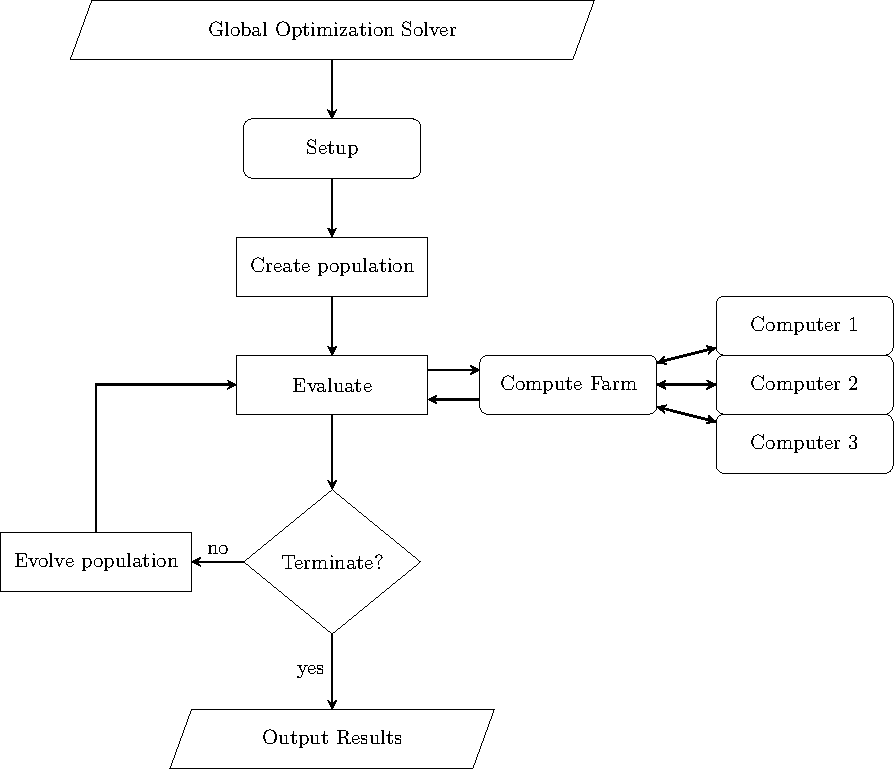
\includegraphics[width=10cm,height=15cm]{chapters/chapter_3_Software/flowchart.pdf}
    \caption{Process of a global optimization algorithm using Computefarm}
    \label{fig:computefarm}
\end{figure}
Computefarm will take a list of population points and distributed them out to various client computers that will then return a result list to global optimization algorithm to further proceed in the optimization process. In this thesis Computefarm is applied to PSO to solve the applications in Chapter \ref{applications}, by taking Alg. \ref{algorithmPSO} an altered algorithm is implementd to use Computefarm Alg. \ref{CFPSO}.

\begin{algorithm}[H]
  \begin{algorithmic}[2]

      \State \textbf{initialize} Computefarm \Comment{initializes the setup of the software}
    \For{each particle i}
        \State \textbf{initialization} $x_i$, $v_i$, $xbest_i$ \Comment{random value for $x_i$ and $v_i$}
        $xbest_i \gets xbest_i$
    \EndFor
    \State \textbf{Evaluate} Computefarm(X) \Comment{evaluate the list of points X using Computefarm}
    \For{each particle i}
        \State \textbf{Update} $xbest_i$ \Comment{update if $f(x_i) < f(xbest_i)$}
    \EndFor
    \While{not termination condition}
        \For{each particle i}
            \State \textbf{update} xglobal \Comment{update if $f(xglobal) < f(xbest_i)$}
            \State \textbf{calculate} $v_i$ \Comment{Using one of the PSO velocity equations}
            \State $x_i = x_i + v_i$
        \EndFor
        \State \textbf{Evaluate} Computefarm(X)
        \For{each particle i}
            \State \textbf{update} $xbest_i$
        \EndFor
    \EndWhile
  \end{algorithmic}
\caption{ComputeFarm Particle Swarm Optimization}
\label{CFPSO}
\end{algorithm}
 
This algorithm is applied in the PSO variants in the software \textit{pythOPT}, a problem solving environment, creating a distributed PSO version called Computefarm Particle Swarm Optimization (CFPSO).

To further understand the implementation steps taken in Computefarm, Figure \ref{fig:implementation} shows the overall design of the distributed system. 

\begin{figure}[h!]
    \centering
    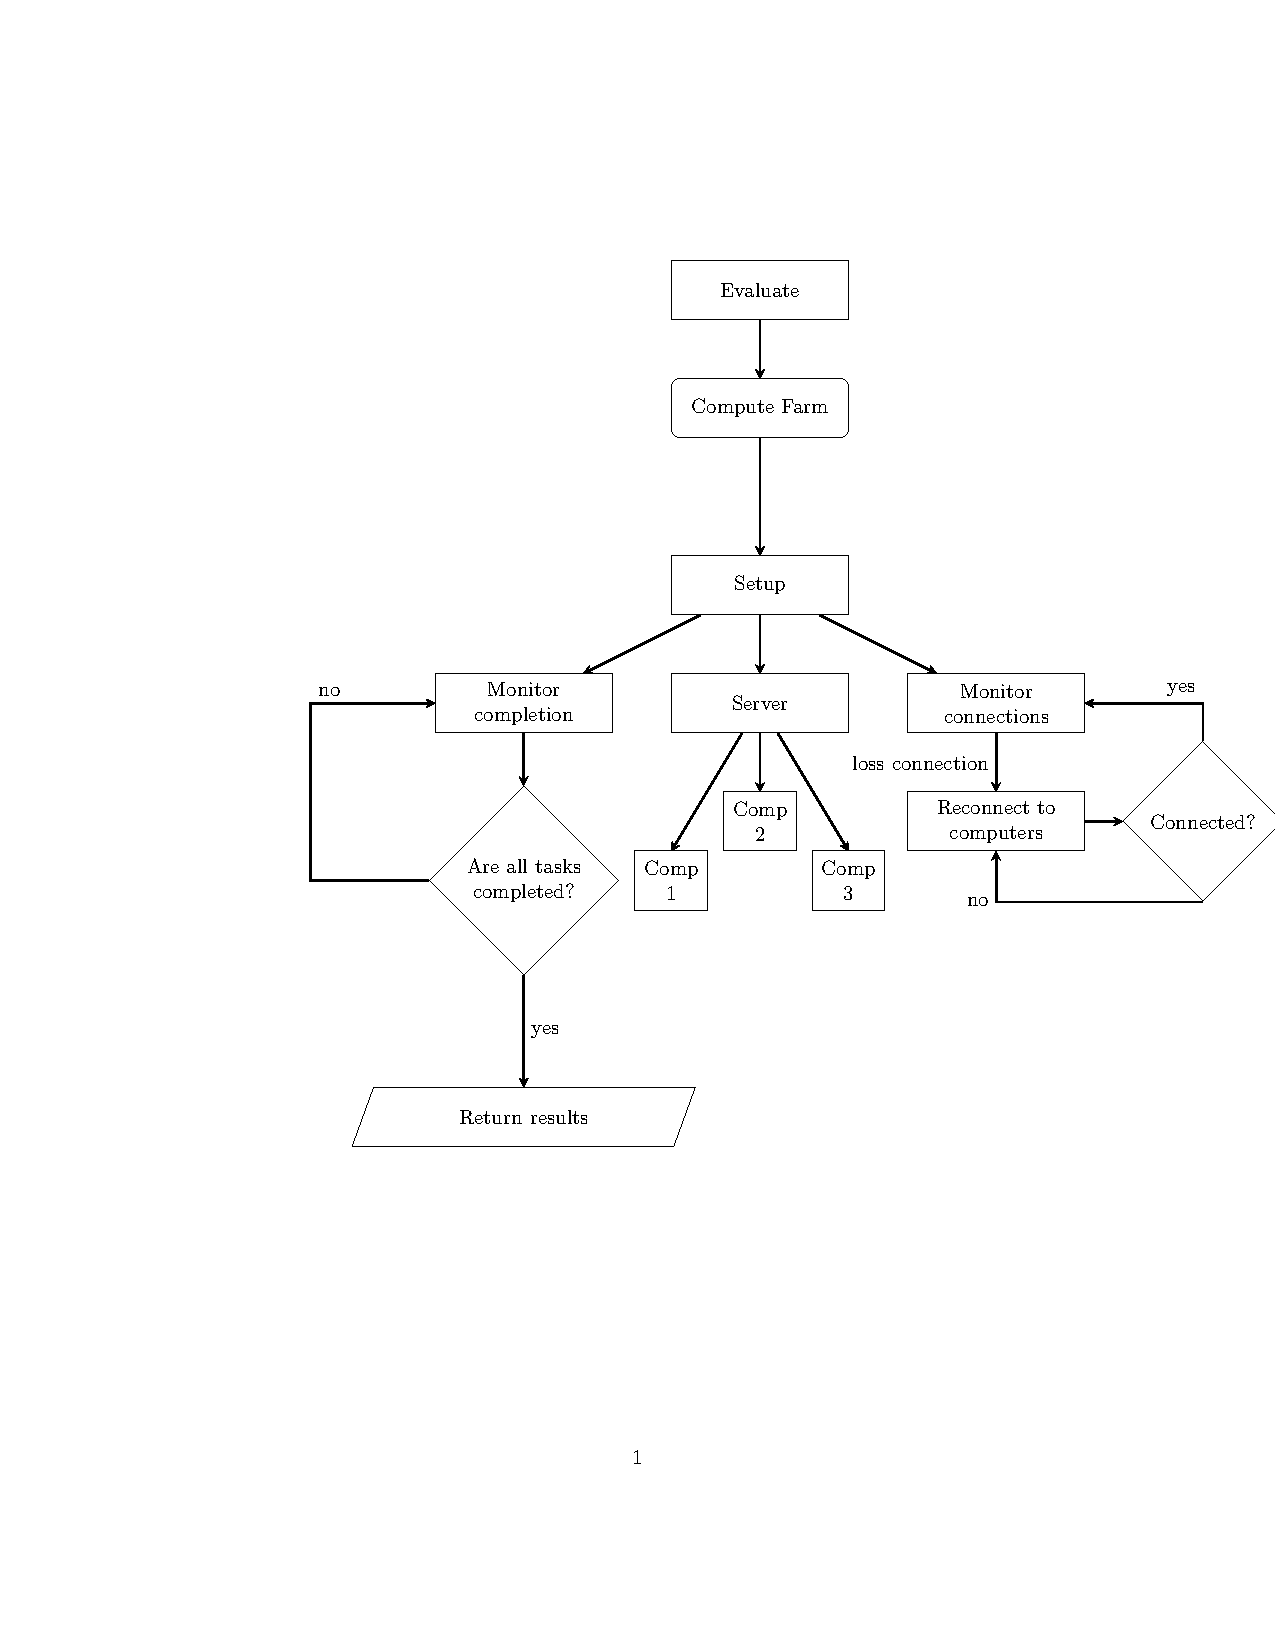
\includegraphics[width=10cm,height=10cm]{chapters/chapter_3_Software/flowchart2.pdf}
    \caption{Process of a global optimization algorithm using Computefarm}
    \label{fig:implementation}
\end{figure}

During the setup phase of Computefarm, three POSSIX \textit{threads} are used to run the functions
\begin{itemize}
    \item Monitor completion,
    \item Server, and
    \item Monitor connections. 
\end{itemize}

Threads are used in this software because of the shared memory properties they have that allows for a form of message passing in the program. Each thread function takes care of a single process that monitors a list to determine further actions. The lists that are shared in memory between the three threads are the medium for message passing in program. 

Monitor completion function takes care of monitoring if all tasks are completed before returning the results to solver. The Server function creates a TCP socket and binds to any client computers communicating on the same port. TCP sockets were chosen because of their reliable connection handling. Threads are generated for each connected client to allow for concurrency in the server system. Each connection is handled by connection handler that will assign itself to a client
machine by receiving the hostname of that machine. Once this is obtained the connection handler will change an client assigned flag for that machine from zero to one. After this it will continuously monitor particle list that contains a particle information structure. The particle information
structure contains the following information 
\begin{itemize}
    \item particle number,
    \item particle position,
    \item function value,
    \item length of position, 
    \item assigned flag, and
    \item completion flag.
\end{itemize}
While monitoring the particle list, if any particle is not assigned to a connection handler then it will change the assigned flag from zero to one indicating it has been assigned. To ensure multiple connection handlers do not assign themselves the same particle \textit{mutexs} are used to ensure mutual exclusion. Once a connection handler has assigned itself a particle, it will then send the particle position information to the client computer using the TCP socket. Because this portion
of the program is written in programming language C, the particle position array length is also stored and sent to the client computer. The connection handler will then wait to receive a message from the client. This message will contain the resulting function evaluation. The connection handler will then store the function value for the specific particle and change the finished flag from zero to one. In the case of disconnect of the client, the connection handler will de-assign itself from
the particle by changing the assigned flag back to zero, changed the client assigned flag back to zero and exit. The work flow of the connection handler is described in the following Figure \ref{fig:connection handler}.

\begin{figure}[h!]
    \centering
    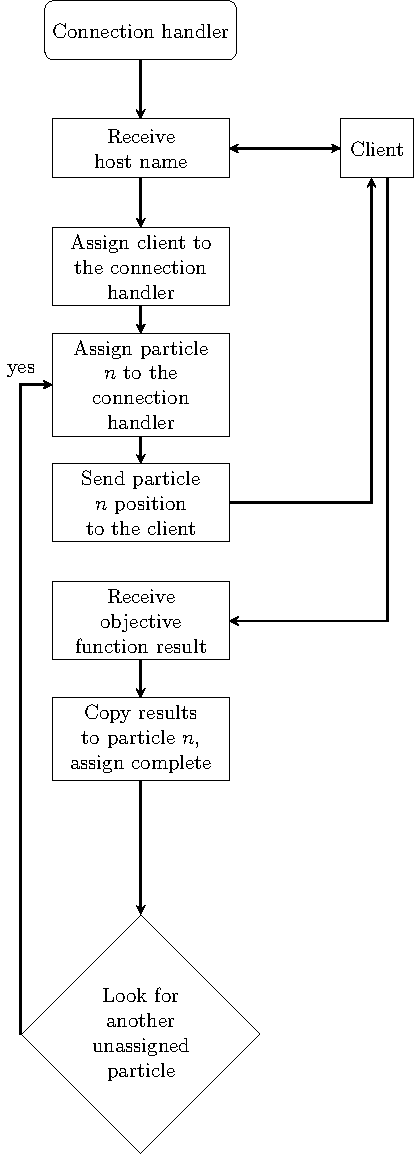
\includegraphics[width=8cm,height=10cm]{chapters/chapter_3_Software/connection_handler.pdf}
    \caption{Computefarm connection handler work flow}
    \label{fig:connection handler}
\end{figure}

The Monitor connection function awakens client machines to run the client script to connect to the server and monitor any machines that disconnect. When machines disconnect a separate thread function, reawaken clients, will attempt to awaken any known disconnected machines every $N$ minutes (default ten minutes). This ensure the maximum number of client machines connected to the server every $N$ minutes from start up. Disconnected machines are determined by assigned flag in client
structure that contains the host name of the machine  and assigned flag. When the assigned flag is zero the reawaken function will attempt to awaken that client machine. 

In the following second phase of Computefarm the Server and Monitor connections threads will be kept alive while the Monitor completion will be called by the solver. The Monitor completion function will re-initialize the particle list with new positions and reset all other information on the particle, the following process of the Server and Monitor connections will continously run to complete all function evaluations. Once every particle is evaluated then the Monitor completion will return
the results back to the solver. This phase will be repeated multiple times until the final phase. 

The final phase is when the solver is done its optimization process and is terminating. To ensure no leakage of memory or zombie threads, a termination function will be called by the solver to terminate all threads and running processes with in Computefarm. 


\section{Optimization Database}
\label{database}
\subsection{Inspiration}
The Optimization Database is used to deal with various challenges present in the global optimization process. One challenge is monitoring the optimization process and if the problem is solved. Because global optimization solvers run until a termination condition is satisfied, a solution could be found sooner than later. Thus a Standard method of monitoring the optimization process is having the best value at each iteration step printed or saved in a log file. This can become
unreliable if the file cannot save or printed values are lost to due to a failure. Also sorting through printed out information or files can be a lengthy process or needs extra code to do so. A way around this is using a database to store values based a policy. In the Optimization database there
are three policies the user can chose from
\begin{itemize}
    \item best value, 
    \item every evaluation, or
    \item evert $n$th evaluation.
\end{itemize}
The database will store values based on the policy chosen at each evaluation and when inserted into the database it ensure the transaction is completed. If the transaction does fail it will report an error and try two more times to reconnect and insert the data. If this does not more then it will send a warning message to the user and continue the optimization process. 
Some situations when monitoring is need is when 
\begin{itemize}
    \item premature convergence occurs, 
    \item performance testing, or
    \item obtained results.
\end{itemize}

Another challenge of global optimization is interest of obtaining $N$ best solutions, because global optimization is implemented to solve for the global minimum it is unusual to have a solver that returns the $N$ best global solutions. Therefore the Optimization database is used to sort through the data and obtain the $N$ best solutions that the solver explored. This becomes useful in the Chapter \ref{rational design} for the crystal structure prediction problem where there are
metastable crystal structures. The metastable structures are of an interest because they can also have interesting properties. An example of this is diamond, it is a metastable structure to Carbon with the stable structure being graphite. In a global optimization, graphite is the global minimum because it has the lowest total energy. However, diamond being the second lowest energy has the property of being very hard and used in multiple research experiments to define hardness and compare
hardness to other structures. Thus the Optimization Database is used to obtain the $N$ lowest energy crystal structures for various compounds. Another data storing problem of global optimization is obtain extra information on the objective function. The extra information can be
\begin{itemize}
    \item information on the data, for example the symmetry group of a predicted crystal structure, or
    \item sorting information on various instances, for example the time duration it takes to correct for errors in a quantum component discussed in Chapter \ref{qubit}.
\end{itemize}
The Optimization database is used to store information on the optimization of the objective function and be flexible to the user to change storage policies and store extra information. This allowing for easier, reliable data collection on the global optimization process.
\subsection{Requirements}

The Optimization Database is used to store information for optimization problems, this includes local and global solvers. In this thesis the database is used only for global optimizations. The database software as primarily one user case, to store information about the global optimization. It is implemented to setup and create tables for users will no prior knowledge of databases and it can change what information is stored in the tables. The primary information needed is
\begin{itemize}
    \item PostgreSQL database information, 
    \item Problem name, and 
    \item global optimization settings.
\end{itemize}

\subsection{Schema}

The Optimization Database is implemented for users with no prior knowledge of databases. On use of the software it will create a local PostgreSQL database if the user does not have a local or remote database setup. It will then automatically setup two tables, settings and problem table. The settings table stores information about the settings used for the global optimization with the default columns
\begin{itemize}
    \item global optimization method,
    \item lower bound,
    \item upper bound,
    \item seed, and
    \item note on simulation. 
\end{itemize}
Columns that are included and maintained by the database is
\begin{itemize}
    \item primary key id,
    \item status, and 
    \item check in time. 
\end{itemize}
The primary key is used to associate any instance of the problem that will be storing its data in the problem table. The status column is updated by the software to keep status if a simulation is still running. Whenever the database is updated or inserted into, the check in time will be automatically updated to the current time. This check in time can later be used to determine if the simulation has been running for the past $N$ hours. In combination with a automatic email component to the
software the user can be notified on result and the status of the optimization daily. 

The problem table is the record of data on the objective function that by default stores
\begin{itemize}
    \item Foreign key id,
    \item $x$ position,
    \item $f$ (function evaluation result),
    \item evaluation number, and
    \item insertion time.
\end{itemize}
The user can also chose to have extra columns to store other data about the objective function. As mentioned before this can be used for quicker sorting methods between instances or properties of the simulation. 

Figure \ref{fig:database schema} represents the database schema used by the software where one settings table has multiple instances of problem tables. 


\begin{figure}[!h]
    \centering
    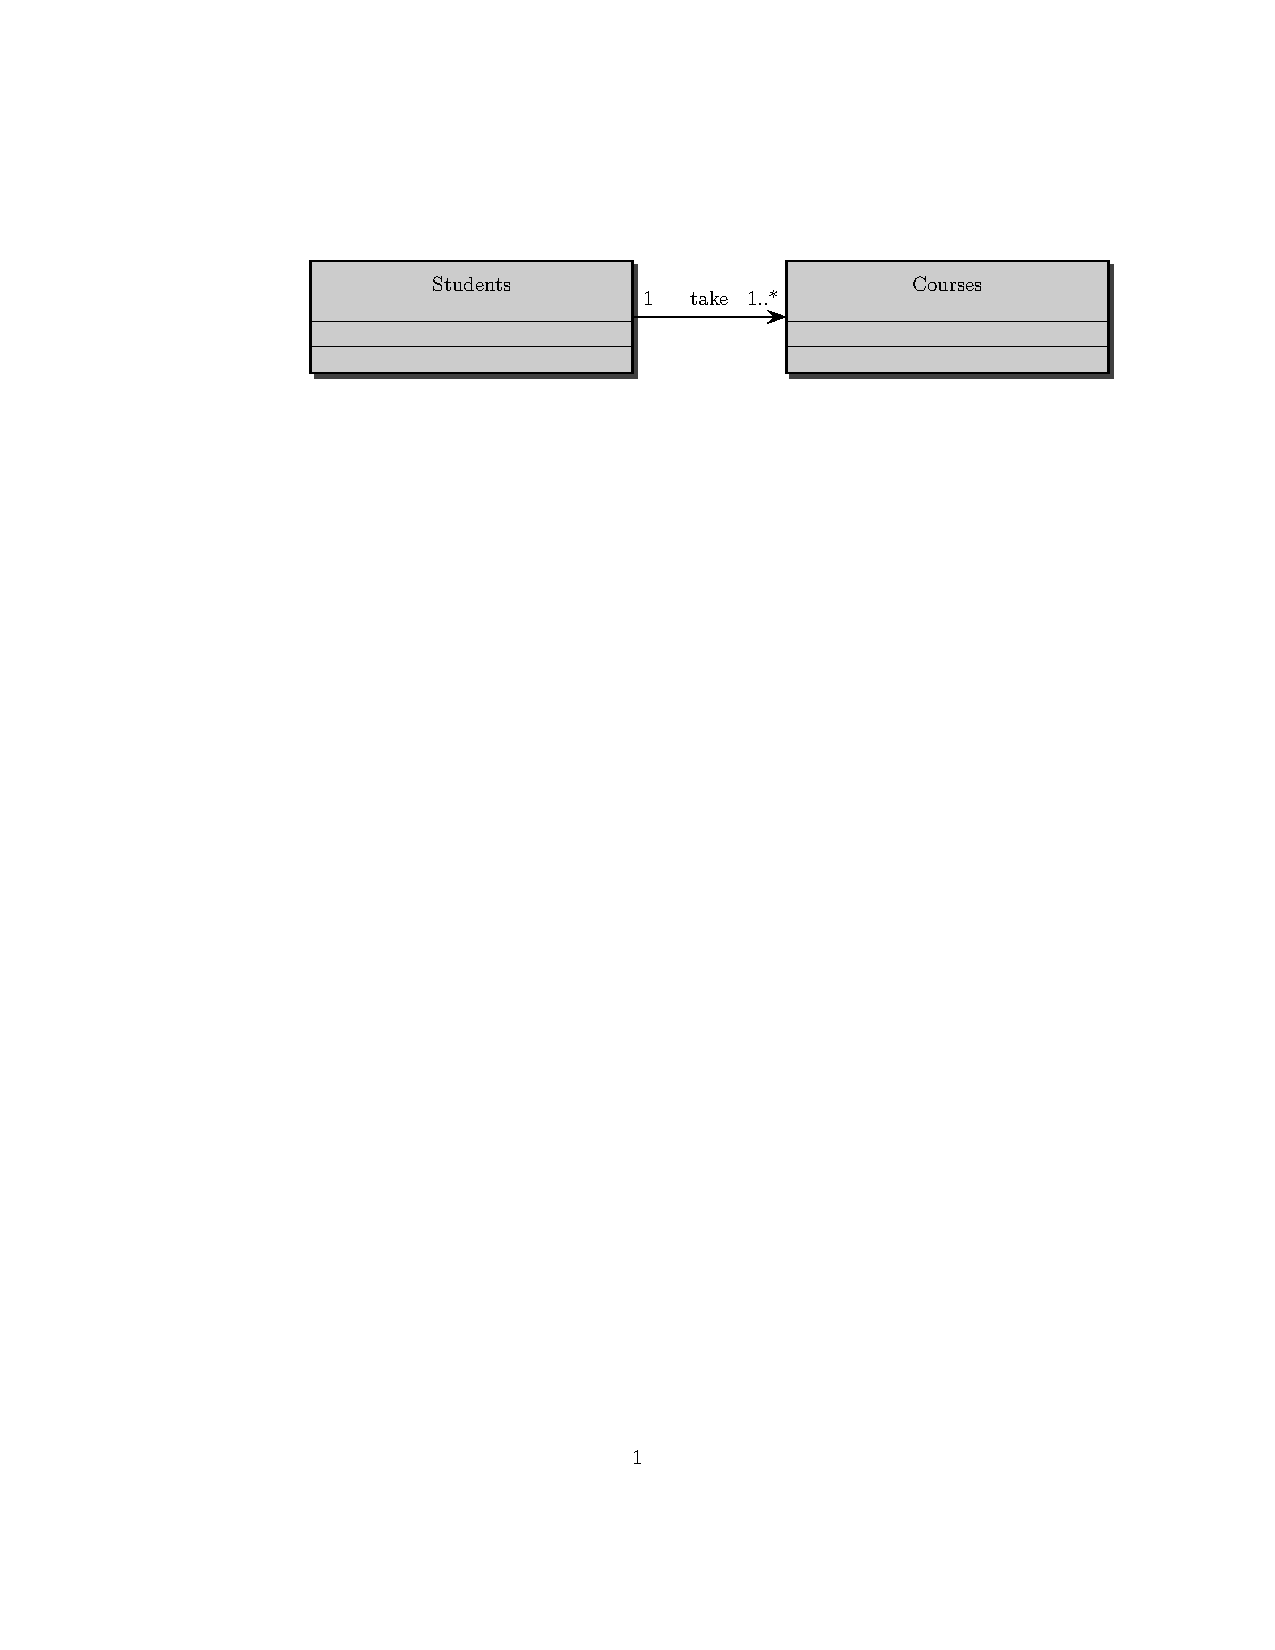
\includegraphics[width=5cm]{chapters/chapter_3_Software/database_schema.pdf}
    \caption{Optimization Database schema.}
    \label{fig:database schema}
\end{figure}




